
% Nesta construção do compilador, foi feita análises léxica manualmente através de loops mudando o estado atual para separada a entrada, que seria um string do arquivo inteiro, para uma lista de tokens. Já a análise sintática usamos a gramática livre de contexto \autoref{@@@} para nos guiar, somado a tabela de precedencia para aplicamo o Pratt Parsing que resulta em uma AST.



% Why pratt is better:
%
% MultiplicativeExpr = MultiplicativeExpr * AddExpr
% AddExpr = AddExpr * Expr
%
% no prat parsing a regra de derivação é a mesma , adicionado de uma tabela
% Expr = Expr (*|+) Expr

% Primeiro foi criado o analisdor lexico, um pacote inteiro para esse analisador na linguagem odin. O trabalho desse analisdor é transform um array de caracteres que é a entrada e retonar uma sequencia de tokens. Cada token tem um tipo ( chamado de kind em código), um valor, reservado para numeros, texto, e posição, que é usado para reportar erros.

% Cada tipo (\textit{kind}) é cado pela enumeração \textbf{Token\_Kind}, essa encoda todos os possiveis tipos comomo dito @{cite previous chapter talking about the entry language}.
% Esses token podem ser: comentarios gerados por uma linha que comece com \%, números, identificadores que são qualquer sequencia de caractheres que não seja palavras especiais, simbolo de igual ('='), simbolos de operadores ('\^', '*') .. bla, funções espciais ($\max$, $\sin$, $\arccos$, etc ...)
%
%
% \begin{codigo}[H]
%   \caption{\small } \label{}
% \begin{lstlisting}
% Token :: struct {
%     kind: Token\_Kind,
%     val: union{i64,f64},
%     text: string,
%     pos:  Position,
% }
%
% \end{lstlisting}
% \end{codigo}
%
% O processo de lexing feito com um loop, simulado a uma maquina de estados, que decide qual token deve ser criado em sequencia ao olhar o caractere atual e o estado.
%
% Estados estão relacionados ao processo de identificar estados pode estar relacionados a identificar palavras.
%
% É  adiante, por exemplo se encontrar um um '1' sabemos que é um numero, podendo ter um '.' para indicar decimal, então utilizamos 
% uma subrotina para identificar esse continuar processando o "input" até o token de numeros ter sido totalmente coletado, se no meio de processar um número um caractere não esperado for encontrado, reportamos um error léxico, exemplos pode ser visto na imagem @{Mostre Imagem com Erro}
% O mais simples são tokens de um caractere '\^', '*', '/', '+', '-', '?', '=', '~', '(', ')', ',', ':', '{', '}', '\_', cara um tem um proposito especifico na analise lexica. Na etapa lexica nos preopados apenas em separar nos tokens de maneira cega ao seu significado.
%
%
% Todo identificador, especial ou não é processado da mesma maneira, é verificado se o caractere atual é um letra ou um '\\', isso indica o começo 
% de um identificador. Depois de de
%
% A gramatica dos tokens é regular e será representada abaixio:
%
%
% Vale ressaltar que nesse moment é criado uma tabela que mapeia cada numero de linha à um string dessa mesma linha, para reportar error, printando a linha do problema mais a linha anterior e posterior para.
% Tem um token que é especial que indica o começo de um ambiente `\\begin{equation}`, qualquer comentario antes de apaerecer esse token é ignorado, isso é para poder dar como entrada ao compilador um documento inteir ocontendo begin document e ainda funciojnar
%
%
%
% \subsection{Analise Semantica}
%
% \subsubsection{Tabela de Symbolos}
% Symbolos podem ser declarados fora de ordem, ciramos um grafo de dependencias e fazemos um orednação topologica de dependencia.
% Isso é póis, ao detectar analisa um certo symbolo queremos dizer se está usando simbolos não definidos, para isso precisamos definifir todos os simbolos glocais que estão no escopo visivel à todos, isso incluisimbolos pre-definidos pela linguagem, (ver tabela @{tabela de simbolos predefinidos}, para isso precisamos primeiro primeiro coletar todos esses e analisar priomeiros oq que dependen de ninguem, e medida que tão
% . Também pode ocorrer dependecia circular sem reoslução e nesse caso reportamos um erro, nesse caso precisamos. @{true? ciruclar dependency?}
%
% \subsubsection{Inferencia de Tipos}
%
% \subsection{SVG da arvore abstrata com inferencia de tipos}
% Para identificar possiveis erros de ordenação algumas medidas foram feitas para auxiliar, como a geração de uma imagem da
% em SVG da arvore sintatica, já com inferencia de tipos


\section{Análise Léxica (\texttt{lexer})} \label{section-lexer}

Nesta etapa, é realizado o processo de tokenização de um subconjunto dos simbolos possiveis no ambiente de equação do \LaTeX{}, como comentado na \autoref{especificacao-linguagem}. A entrada desse processo são os caracteres do arquivo fonte, enquanto a saída é uma sequência lógica desses caracteres, organizada em \textit{tokens}. O código responsável por essa funcionalidade está contido no pacote \texttt{lexer}.

O processo de tokenização realiza uma varredura completa no arquivo de entrada, caractere por caractere, para identificar e extrair os \textit{tokens}. Antes de iniciar essa extração, verificamos se o trecho analisado pertence a um ambiente de equação. Essa verificação é feita ao identificar a string (cadeia de caracteres) \verb|\begin{equation}|, que marca o início da extração de \textit{tokens}. Da mesma forma, a delimitação do ambiente se encerra com a string \verb|\end{equation}|. Isso permite que o sistema ignore partes do arquivo que não pertencem ao ambiente de equação, como textos explicativos ou outros elementos presentes no mesmo arquivo \texttt{.tex}. Dessa forma, garantimos que a tokenização seja restrita às seções relevantes do código.

Para fins de documentação e maior clareza, definimos uma gramática formal que descreve a geração dos \textit{tokens}, apresentada na \autoref{grammar-tokens}. O alfabeto dessa gramática é composto pelos caracteres do arquivo fonte. Apesar de documentar com uma gramatica, a geração dos \textit{tokens} é implementada internamente de maneira semelhante à simulação de uma máquina de estados.

Na definição da gramática (\autoref{grammar-tokens}), utilizamos uma notação leve de sintaxe para representar suas regras. Palavras com todas as letras minúsculas representam não-terminais, enquanto palavras entre aspas simples correspondem a caracteres literais específicos. Por outro lado, palavras em letras maiúsculas denotam categorias semânticas, como \texttt{DIGIT}, que representa qualquer dígito de 0 a 9, e \texttt{LETTER}, que cobre letras de \texttt{'a'} a \texttt{'z'}.

Ainda, definimos símbolos operadores: ``$*$'' indica zero ou mais ocorrências; ``$()$'' indica agrupamento para aplicar um operador ao mesmo; ``$|$'' simboliza o início de uma regra alternativa para o mesmo não-terminal, ou se estiver dentro de um agrupamento, como por exemplo``$(a|b)$'', significa que aceita $a$ ou $b$; e ``$=$'' indica uma produção. Essa mesmta sintaxe de gramática é utilizada na análise sintática, onde cada regra é faz bijeção com os tipos de nó da AST, como detalhado na \autoref{section-parser}. Nessa etapa seguinte, o alfabeto passa a ser composto pelo conjunto de \textit{tokens} gerados.

%%%%%%%%%%%%%

O pacote inteiro de tokenização pode ser acessado por meio de uma única função, descrita na \autoref{function-lex}, escrita na linguagem \texttt{Odin}. Essa função, chamada \texttt{lex}, aceita uma lista de caracteres como entrada e retorna uma lista de estruturas do tipo \texttt{Token} (detalhado na \autoref{lexer-structs}). A estrutura \texttt{Token} possui três campos principais:

\begin{itemize}
    \item \texttt{kind}: identifica o tipo de \textit{token}, mapeando-o para uma das regras de produção definidas na \autoref{grammar-tokens}.
    \item \texttt{text}: contém a string correspondente ao \textit{token} gerado.
    \item \texttt{position}: uma instância do tipo \texttt{Position}, que registra a posição exata do \textit{token} no arquivo de origem.
\end{itemize}


\begin{codigo}[htb]
        \caption{\small Função principal do Lexer. }
        \label{function-lex}
  \begin{lstlisting}[language = c]
  
    lex :: proc(input: []u8) -> []Token
  \end{lstlisting}
\end{codigo}



Durante a iteração sobre o \texttt{input}, o processo de tokenização mantém algumas variáveis de controle para monitorar o estado do fluxo de caracteres. Quebras de linha são contadas ao encontrar sequências como \verb|"\n"| ou \verb|"\n\r"|. É mantida a coluna atual que rastreia a posição horizontal do caractere em uma linha. O cursor é o índice que aponta para o caractere atualmente em processamento. Essas informações são usadas para preencher o campo \texttt{position} de cada \textit{token}, uma funcionalidade essencial para a geração de relatórios de erro. A estrutura \texttt{Position}, detalhada na \autoref{lexer-structs}, armazena essas informações para garantir a precisão no rastreamento de problemas.

O sistema de relatório de erros, implementado nesta etapa, é utilizado de forma consistente por todos os pacotes do projeto. Essa funcionalidade assegura que erros sejam associados a posições específicas no arquivo de entrada, facilitando a depuração e correção. A assinatura da função de tratamento de erros, bem como suas possíveis variações, está documentada na \autoref{function-errors}.


\begin{codigo}[htb]
    \caption{\small Função de erro exposto pelo pacote \texttt{lexer}. }
        \label{function-errors}
\begin{lstlisting}[language=C++]
error_from_pos :: proc(pos: Position, msg: string, args: ..any)
error_from_token :: proc(token: Token, msg: string, args: ..any);
\end{lstlisting}.
\end{codigo}.


\subsection{Reporte de Erros} \label{subsection-erros}


Dada uma posição ou um \texttt{token}, é exibido uma mensagem (\texttt{msg}) diretamente no terminal, formatada para destacar visualmente o erro em vermelho. A formatação utiliza as informações do \texttt{token}, como o nome do arquivo, linha, coluna e comprimento do \texttt{token} problemático, permitindo sublinhar precisamente onde o erro ocorreu. Isso proporciona maior clareza nas mensagens de erro, como exemplificado no caso de erro semântico de uso de identificadores não definidos (\autoref{error-undefined-symbol}).

Outros exemplos de erros seguem o mesmo padrão de exibição e incluem: tipos incompatíveis (\autoref{error-incompatible-types}), símbolos não definidos (\autoref{error-undefined-symbol}), balanceamento de parênteses (\autoref{error-balanceamento}), uso de palavras reservadas (\autoref{error-reserved-word}) e \textit{tokens} que não formam uma expressão matemática válida (\autoref{error-cant-make-expression}).
    


\begin{figure}[H]
    \caption{\label{error-undefined-symbol} \small Erro ao usar simbolo não definido.}
    \begin{center}
        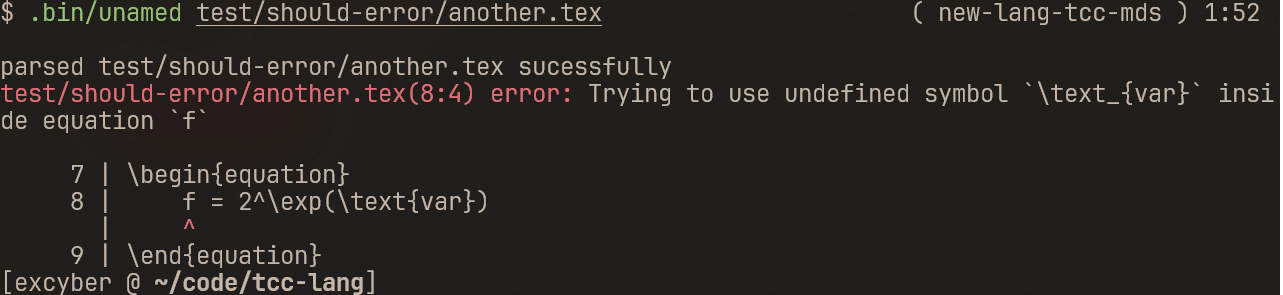
\includegraphics[scale=0.5]{./Imagens/error-undefined-symbol.png}
    \end{center}
\end{figure}

\begin{figure}[H]
    \caption{\label{error-incompatible-types} \small Erro de de tipos incompativeis.}
    \begin{center}
        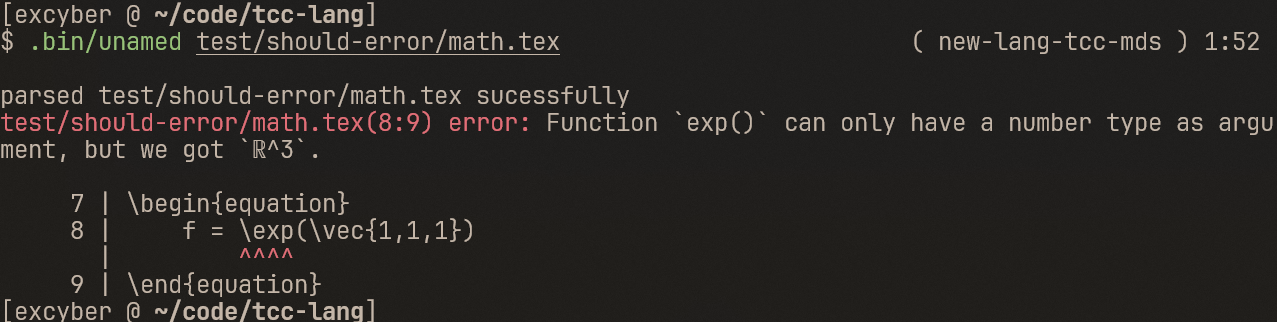
\includegraphics[scale=0.5]{./Imagens/error-incompatible-types.png}
    \end{center}
\end{figure}


\begin{figure}[H]
    \caption{\label{error-balanceamento} \small Erro de balanceamento de parentesis.}
    \begin{center}
        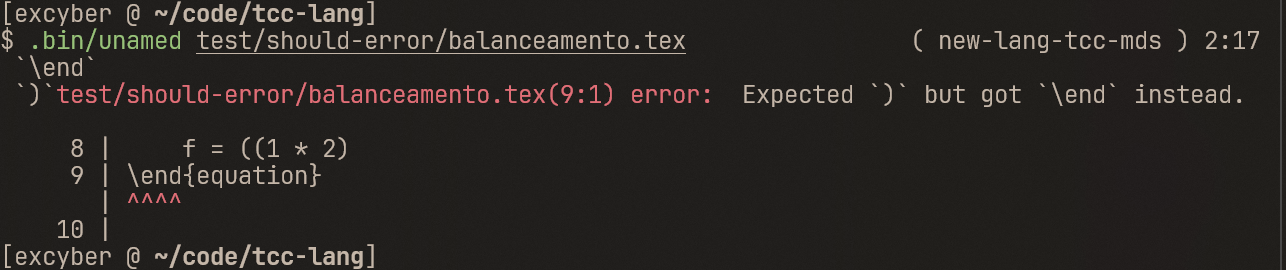
\includegraphics[scale=0.5]{./Imagens/error-balanceamento.png}
    \end{center}
\end{figure}

\begin{figure}[H]
    \caption{\label{error-reserved-word} \small Erro de uso incorreto de palavras reservadas.}
    \begin{center}
        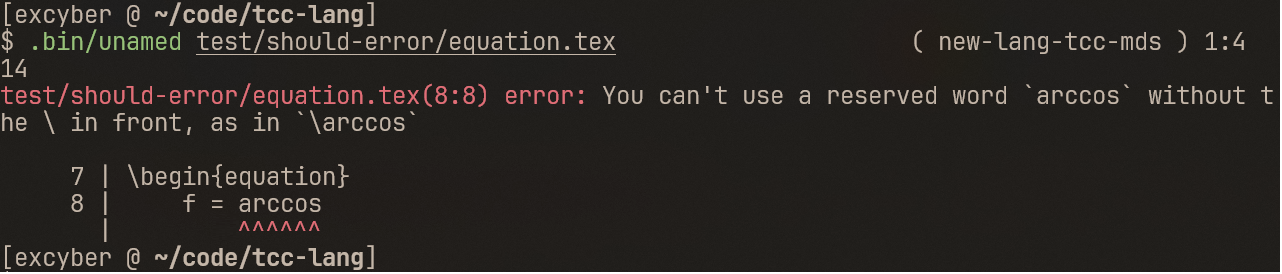
\includegraphics[scale=0.5]{./Imagens/error-reserved-word.png}
    \end{center}
\end{figure}


\begin{figure}[H]
    \caption{\label{error-cant-make-expression} \small Erro de \textit{token} incapaz de produzir expressão.}
    \begin{center}
        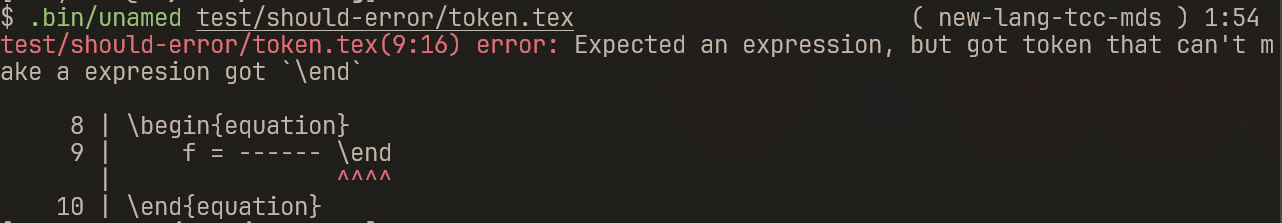
\includegraphics[scale=0.5]{./Imagens/error-cant-make-expression.png}
    \end{center}
\end{figure}


\subsection{Classificação e Extração de Tokens}


Tokens simples, como aqueles compostos por um ou dois caracteres, são extraídos lendo-se o número correspondente de caracteres do \texttt{input}. Após a leitura, o \texttt{token} é construído e o laço continua para o próximo. Quando um caractere \texttt{\%} é encontrado, os caracteres subsequentes são ignorados até a próxima quebra de linha. Isso adiciona suporte a comentários no estilo \LaTeX{}.

Tokens mais complexos, como números, identificadores ou \textit{tokens} especiais, são extraídos com base em suas características. Números podem opcionalmente conter um ponto decimal, como em $1.0$. Já identificadores consistem em uma ou mais letras, opcionalmente prefixadas pelo símbolo \verb|\|.

A gramática de \textit{tokens} provida é intrinsecamente ambígua. Por exemplo, uma sequência como \verb|\frac| pode ser interpretada como um identificador comum ou como \verb"token\_frac". Para resolver essa ambiguidade, criamos um dicionário que mapeia identificadores especificos para \textit{tokens} especiais (\autoref{map-special-identifiers}). Assim, se um identificador começar com o caractere \verb|\|, ele será verificado no dicionário e classificado como um token especial, se apropriado.


\label{lexer-subexpression}
Identificadores não permitem números nem mesmo o caractere de sublinhado (\verb|_|). Isso ocorre porque, no analisador sintático, um nó do tipo identificador é modelado como um tipo recursivo, permitindo que identificadores sejam aninhados ao conter outros nós. Dessa forma, não é necessário permitir sublinhados diretamente no nível de token, o que possibilita a escrita de identificadores mais complexos, como \verb|\pi{n_1}| (renderizado em \LaTeX{} como $\pi_{n_1}$). Nesse caso, \verb|\pi| seria o primeiro token do nó identificador, e sua subexpressão seria \verb|n_1| (renderizado como $n_1$), que, por sua vez, é o identificador \verb|n| com a subexpressão \verb|1|.

Adicionalmente, permitimos o uso da palavra-chave \verb|\text|, como em \verb|\text{id}|, para descrever identificadores. Essa palavra-chave é utilizada para incluir texto dentro do ambiente de equações em \LaTeX{}, proporcionando maior flexibilidade na representação e manipulação de identificadores. A extração desse token segue um processo semelhante ao do suporte para \verb|\vec{id}|.

A enumeração que representa os tipos de tokens pode ser consultada na \autoref{enum-token-kind}. Cada entrada dessa enumeração corresponde diretamente às regras de produção definidas na gramática apresentada na \autoref{grammar-tokens}. Para facilitar a leitura, adicionamos, à direita de cada entrada, o símbolo que a representa, indicado em comentários.

Com a etapa de tokenização concluída, avançamos para a análise sintática, onde exploramos como os \textit{tokens} gerados são organizados em estruturas hierárquicas que formam a árvore sintática.

\begin{codigo}[htb]
        \caption{\small Estuturas do Lexer. }
        \label{lexer-structs}
\begin{lstlisting}[language=C++]

Token :: struct {
    kind: Token_Kind,
    val: union{i64,f64},
    text: string,
    pos:  Position,
}

Position :: struct {
    file:   string,
    offset: i64,   // starting at 0, buffer offeset in file
    line:   i64,   // starting at 1, starting
    column: i64,   // starting at 1
    length: int    // how much chars foward
}
    
  \end{lstlisting}
\end{codigo}


\begin{codigo}[htb]
        \caption{\small Mapa de indentificadores especiais. }
        \label{map-special-identifiers}
  \begin{lstlisting}[language=C++]

SPECIAL_WORDS := map[string]Token{
    "text"  = Token{text = "\\text",     kind =.Text},

    // Special
    "frac"   = Token{text = "\\frac",    kind =.Frac},
    "vec"    = Token{text = "\\vec",     kind =.Vec},
    "cdot"   = Token{text = "\\cdot",    kind =.Mul},
    "begin"  = Token{text = "\\begin",   kind =.Begin},
    "end"    = Token{text = "\\end",     kind =.End},
    "rho"    = Token{text = "\\rho",     kind =.Rho},
    "sqrt"   = Token{text = "\\sqrt",    kind =.Sqrt},
    "omega"  = Token{text = "\\omega",   kind =.Omega},

    // Cross product
    "times"  = Token{text = "\\times",   kind =.Cross},

    "max"    = Token{text = "\\max",     kind =.Max},
    "min"    = Token{text = "\\min",     kind =.Min},
    "exp"    = Token{text = "\\exp",     kind =.Exp},

    "cos"    = Token{text = "\\cos",     kind =.Cos},
    "sin"    = Token{text = "\\sin",     kind =.Sin},
    "tan"    = Token{text = "\\tan",     kind =.Tan},

    "arccos" = Token{text = "\\arccos",  kind =.ArcCos},
    "arcsin" = Token{text = "\\arcsin",  kind =.ArcSin},
    "arctan" = Token{text = "\\arctan",  kind =.ArcTan},

    "theta"  = Token{text = "\\theta",   kind =.Theta},
    "phi"    = Token{text = "\\phi",     kind =.Phi},

    "alpha"   = Token{text = "\\alpha",  kind =.Alpha},
    "beta"    = Token{text = "\\beta",   kind =.Beta},
    "sigma"   = Token{text = "\\sigma",  kind =.Sigma},
    "pi"      = Token{text = "\\pi",     kind =.Pi},
    "epsilon" = Token{text = "\\epsilon",kind =.Epsilon},
}

    
  \end{lstlisting}
\end{codigo}


\begin{codigo}[htb]
    \caption{\small Gramatica ilustrativa para \texttt{tokens}. }
        \label{grammar-tokens}
  \begin{lstlisting}[numbers=none, frame=none, language=haskell]

    token_number     = DIGIT DIGIT* '.' DIGIT DIGIT* | DIGIT DIGIT*;
    token_identifier = '\' LETTER LETTER* | LETTER LETTER*;
    token_cmpgreater = '>';
    token_cmpless    = '<';
    token_cmpequal   = '==';
    token_equal      = '=';
    token_mul        = '*' | '\cdot';
    token_cross      = '\times';
    token_div        = '/';
    token_plus       = '+';
    token_minus      = '-';
    token_caret      = '^';
    token_semicolon  = ';';
    token_comma      = ',';
    token_colon      = ':';
    token_question   = '?';
    token_bang       = '!';
    token_openparen  = '(';
    token_closeparen = ')';
    token_opencurly  = '{';
    token_closecurly = '}';
    token_tilde      = '~';
    token_underline  = '_'; --- Used for subexpresions
    token_arrow      = '->';
    token_begin      = '\begin';
    token_end        = '\end';
    token_frac       = '\frac';
    token_vec        = '\vec';
    token_omega      = '\omega';
    token_theta      = '\theta';
    token_phi        = '\phi';
    token_rho        = '\rho';
    token_alpha      = '\alpha';
    token_beta       = '\beta';
    token_sigma      = '\sigma';
    token_pi         = '\pi';
    token_epsilon    = '\epsilon';
    token_max        = '\max';
    token_min        = '\min';
    token_exp        = '\exp';
    token_tan        = '\tan';
    token_sin        = '\sin';
    token_cos        = '\cos';
    token_arctan     = '\arctan';
    token_arcsin     = '\arcsin';
    token_arccos     = '\arccos';
    token_sqrt       = '\sqrt';
    token_text       = '\text';
    token_eof        = EOF;
    
  \end{lstlisting}
\end{codigo}



\begin{codigo}[htb]
\caption{\small Enumeração dos tipos de \texttt{tokens}. }
    \label{enum-token-kind}
\begin{lstlisting}[language = C++]
  Token_Kind :: enum {
    EOF           = 0,
    Number,
    Identifier,

    Equal,        // =
    Mul,          // * ou \cdot
    Cross,        // X
    Div,          // /
    Plus,         // +
    Minus,        // -
    Caret,        // ^
    Comma,        // ,
    Colon,        // :
    Question,     // ?
    Bang,         // !
    OpenParen,    // (
    CloseParen,   // )
    OpenCurly,    // {
    CloseCurly,   // }
    Tilde,        // ~
    Underline,    // _
    Arrow,        // ->

    Begin = 256,  // \begin
    End,          // \end

    Frac,         // \frac
    Vec,          // \vec

    Omega,        // \omega
    Theta,        // \theta
    Phi,          // \phi
    Rho,          // \rho
    Pi,           // \pi
    Epsilon,      // \epsilon
    Alpha,        // \alpha
    Beta,         // \beta
    Sigma,        // \sigma

    Max,          // \max
    Min,          // \min
    Exp,          // \exp
    Tan,          // \tan
    ArcTan,       // \arctan
    Sin,          // \sin
    ArcSin,       // \arcsin
    Cos,          // \cos
    ArcCos,       // \arccos
    Sqrt,         // \sqrt

    Text,         // \text
    Invalid
}

\end{lstlisting}
\end{codigo}
